%
% Tallinn University of Technology - bachelor, master thesis Éstonian template for LaTeX
%
%
% Public version 1.4
% 2025 Refactored to follow actual guidelines (Ago Luberg et al.)
%
% Public version 1.3
% 2023 translated main parts to Estonian (by Ago Luberg)
%
% Public version 1.2
% 2022 Updated by Karl Janson to match the new formatting guidelines
%
% Public Version 1.1
% 2019 Adjusted by Frank Korving for his Bachelor Thesis, with contributions from Sander Arnus
%
% Public version 1.0
% 2010 - 2013 Thijs Nugteren and Joos Buijs for Master Thesis
%
% THIS IS THE MAIN FILE (i.e. compile this file, compiling the others directly won't work)
%

\documentclass[12pt]{report} % Default font size is 12pt, default paper size is a4

% all the other includes etc. are done in the thesis.sty file.
\usepackage{thesis} % thesis formatting

%%%%%%%%%%%%%%%%%%%%%%%%%%%%%%%%%%%%%%%%%%%%%%%%%%%%%%%%%%%%%
% NOTE:                                                     %
%%%%%%%%%%%%%%%%%%%%%%%%%%%%%%%%%%%%%%%%%%%%%%%%%%%%%%%%%%%%%
% * Content chapter files are located in "chapters" folder, %
%   included using the "chapters_main.tex" file             %
%                                                           %
% * Appendices are located in "appendices" folder,          %
%   included using the "appendices_main.tex" file           %
%%%%%%%%%%%%%%%%%%%%%%%%%%%%%%%%%%%%%%%%%%%%%%%%%%%%%%%%%%%%%

%%%%%%%%%%%%%%%%%%%%%%%%%%%%%%%%%%%%%%%%%%%%%%%%%%%%%%%%%%%%%
% NOTE:
%%%%%%%%%%%%%%%%%%%%%%%%%%%%%%%%%%%%%%%%%%%%%%%%%%%%%%%%%%%%%
% * config.tex includes automations and variables that are
%   accessible template-wide.
%
% * Author's name, thesis title and other variables must be
%   changed inside the config.tex file.
%%%%%%%%%%%%%%%%%%%%%%%%%%%%%%%%%%%%%%%%%%%%%%%%%%%%%%%%%%%%%
%x%%%%%%%%%%%%%%%%%%%%%%%%%%%%%%%%%%%%%%%%%%%%%%%%%%%%%%%%%%%%
% NOTE: PROCEED WITH CAUTION!
%x%%%%%%%%%%%%%%%%%%%%%%%%%%%%%%%%%%%%%%%%%%%%%%%%%%%%%%%%%%%%
% The commands below need to be defined.
% Square brackets should be removed.
% Estonian title page will be generated automatically       %
%%%%%%%%%%%%%%%%%%%%%%%%%%%%%%%%%%%%%%%%%%%%%%%%%%%%%%%%%%%%%

\newcommand{\lang}{ENG} % Choose the language of the thesis (Estonian is the default one)

% If your work is in Estonian, English title is used for abstract. Don't forget to add it here!
% For English thesis is vice versa
\newcommand{\thesisTitleEng}{Secure Web-Based File Encryption and Management System} % variable with thesis title
\newcommand{\thesisTitleEst}{Secure Web-Based File Encryption and Management System} % Title in Estonian

% Choose your thesis
\newcommand{\thesisType}{ICS0027}

% Thesis author
\newcommand{\authorName}{Kamil Blasiak}
\newcommand{\studentcode}{245156IVSB}

% Second author. If you are the sole author, leave it as it is
\newcommand{\authorNameTwo}{[Second Author name]}
\newcommand{\studentcodeTwo}{[Student Code]}

% Third author. If you are the sole author, leave it as it is
\newcommand{\authorNameThree}{[Third Author name]}
\newcommand{\studentcodeThree}{[Student Code]}

% Main supervisor
\newcommand{\supervisorName}{Ali Ghasempour}
\newcommand{\supervisortitle}{MSc}

% Co-supervisor. If you have only one supervisor, leave it as it is
\newcommand{\cosupervisorName}{[Co-Supervisor's Name]}
\newcommand{\cosupervisortitle}{[Academic degree]}

% Dates. Default to current current date.
% You can hard code a value by replacing the parameter with a text
% Year of publication (defaults to current year).
\newcommand{\Year}{\the\year{}}

% Signature date (defaults to today).
\newcommand{\signatureDate}{\ddmmyyyydate\today}

% PDF Metadata
\newcommand{\version}{Checkpoint 3 draft}
\newcommand{\keywords}{web application security, file encryption, AES-GCM, Argon2id, CSRF, XSS, access control, secure programming}

%%%%%%%%%%%%%%%%%%%%%%%%%%%%%%%%%%%%%%%%%%%%%%%%%%%%%%%%%%%%%
%            DO NOT EDIT BELOW THIS LINE                    %
%%%%%%%%%%%%%%%%%%%%%%%%%%%%%%%%%%%%%%%%%%%%%%%%%%%%%%%%%%%%%

\newcommand{\universityEng}{TALLINN UNIVERSITY OF TECHNOLOGY}
\newcommand{\schoolEng}{School of Information Technologies}
\newcommand{\universityEst}{TALLINNA TEHNIKAÜLIKOOL}
\newcommand{\schoolEst}{Infotehnoloogia teaduskond}

\ifthenelse {\equal{\authorName}{[Author name]}}
  {\newcommand{\authorNameEst}{[Ees- ja perenimi]}}
  {\newcommand{\authorNameEst}{\authorName}}

\ifthenelse {\equal{\studentcode}{[Student Code]}}
  {\newcommand{\studentcodeEst}{[Üliõpilaskood]}}
  {\newcommand{\studentcodeEst}{\studentcode}}

\ifthenelse {\equal{\supervisorName}{[Supervisor's Name]}}
  {\newcommand{\supervisorNameEst}{[Juhendaja nimi]}}
  {\newcommand{\supervisorNameEst}{\supervisorName}}

\ifthenelse {\equal{\supervisortitle}{[Academic degree]}}
  {\newcommand{\supervisortitleEst}{[Teaduskraad]}}
  {\newcommand{\supervisortitleEst}{\supervisortitle}}

\ifthenelse {\equal{\cosupervisorName}{[Co-Supervisor's Name]}}
  {\newcommand{\cosupervisorNameEst}{[Kaasjuhendaja nimi]}}
  {\newcommand{\cosupervisorNameEst}{\cosupervisorName}}

\ifthenelse {\equal{\cosupervisortitle}{[Academic degree]}}
  {\newcommand{\cosupervisortitleEst}{[Teaduskraad]}}
  {\newcommand{\cosupervisortitleEst}{\cosupervisortitle}}

\ifthenelse {\equal{\authorNameTwo}{[Second Author name]}}
  {\newcommand{\authorNameTwoEst}{[Teise autori nimi]}}
  {\newcommand{\authorNameTwoEst}{\authorNameTwo}}

\ifthenelse {\equal{\studentcodeTwo}{[Student Code]}}
  {\newcommand{\studentcodeTwoEst}{[Üliõpilaskood]}}
  {\newcommand{\studentcodeTwoEst}{\studentcodeTwo}}

\ifthenelse {\equal{\authorNameThree}{[Third Author name]}}
  {\newcommand{\authorNameThreeEst}{[Kolmanda autori nimi]}}
  {\newcommand{\authorNameThreeEst}{\authorNameThree}}

\ifthenelse {\equal{\studentcodeThree}{[Student Code]}}
  {\newcommand{\studentcodeThreeEst}{[Üliõpilaskood]}}
  {\newcommand{\studentcodeThreeEst}{\studentcodeThree}}

\ifthenelse {\equal{\thesisType}{Bachelor's Thesis}}
      {\newcommand{\thesisTypeEst}{Bakalaureusetöö}}
      {
        \ifthenelse {\equal{\thesisType}{Master's Thesis}}
          {\newcommand{\thesisTypeEst}{Magistritöö}}
          {\newcommand{\thesisTypeEst}{Bakalaureusetöö / Magistritöö}}
      }

\newcommand{\supervisor}{Supervisor}
\newcommand{\supervisorEst}{Juhendaja}

\newcommand{\cosupervisor}{Co-Supervisor}
\newcommand{\cosupervisorEst}{Kaasjuhendaja}


\ifthenelse{\not \equal{\lang}{ENG}}{
    % Estonian version
    \newcommand{\thesisTitle}{\thesisTitleEst}
    \newcommand{\abstractThesisTitle}{\thesisTitleEng}
    \newcommand{\langEst}{eesti}
    \newcommand{\langEng}{Estonian}
    \newcommand{\selectedLang}{estonian}
    \newcommand{\authorDeclarationTitle}{Autorideklaratsioon}
    \newcommand{\abstactTitle}{Lühikokkuvõte}
    \newcommand{\secondAbstractTitle}{Abstract}
    \newcommand{\listOfTermsTitle}{Lühendite ja mõistete sõnastik}
    \newcommand{\tableOfContentsTitle}{Sisukord}
    \newcommand{\listOfFiguresTitle}{Jooniste loetelu}
    \newcommand{\listOfTablesTitle}{Tabelite loetelu}
    \newcommand{\referencesTitle}{Kasutatud kirjandus}
    \newcommand{\appendixTitle}{Lisa}
    \newcommand{\licenceTitle}{Lihtlitsents lõputöö reprodutseerimiseks ja lõputöö üldsusele kättesaadavaks tegemiseks}
    \newcommand{\licenceFootnote}{Lihtlitsents ei kehti juurdepääsupiirangu kehtivuse ajal vastavalt üliõpilase taotlusele lõputööle juurdepääsupiirangu kehtestamiseks, mis on allkirjastatud teaduskonna dekaani poolt, välja arvatud ülikooli õigus lõputööd reprodutseerida üksnes säilitamise eesmärgil. Kui lõputöö on loonud kaks või enam isikut oma ühise loomingulise tegevusega ning lõputöö kaas- või ühisautor(id) ei ole andnud lõputööd kaitsvale üliõpilasele kindlaksmääratud tähtajaks nõusolekut lõputöö reprodutseerimiseks ja avalikustamiseks vastavalt lihtlitsentsi punktidele 1.1. ja 1.2, siis lihtlitsents nimetatud tähtaja jooksul ei kehti.}
    \newcommand{\abstractPageNumber}{2}
  }{
    % English version
    \newcommand{\thesisTitle}{\thesisTitleEng}
    \newcommand{\abstractThesisTitle}{\thesisTitleEst}
    \newcommand{\langEst}{inglise}
    \newcommand{\langEng}{English}
    \newcommand{\selectedLang}{english}
    \newcommand{\authorDeclarationTitle}{Author’s declaration of originality}
    \newcommand{\abstactTitle}{Abstract}
    \newcommand{\secondAbstractTitle}{Annotatsioon}
    \newcommand{\listOfTermsTitle}{List of abbreviations and terms}
    \newcommand{\tableOfContentsTitle}{Table of contents}
    \newcommand{\listOfFiguresTitle}{List of figures}
    \newcommand{\listOfTablesTitle}{List of tables}
    \newcommand{\referencesTitle}{References}
    \newcommand{\appendixTitle}{Appendix}
    \newcommand{\licenceTitle}{Non-exclusive licence for reproduction and publication of a graduation thesis}
    \newcommand{\licenceFootnote}{The non-exclusive licence is not valid during the validity of access restriction indicated in the student's application for restriction on access to the graduation thesis that has been signed by the school's dean, except in case of the university's right to reproduce the thesis for preservation purposes only. If a graduation thesis is based on the joint creative activity of two or more persons and the co-author(s) has/have not granted, by the set deadline, the student defending his/her graduation thesis consent to reproduce and publish the graduation thesis in compliance with clauses 1.1 and 1.2 of the non-exclusive licence, the non-exclusive licence shall not be valid for the period.}
    \newcommand{\abstractPageNumber}{2}
  }

%
% PDF settings
%
% Packages and styles for the diagrams in the report
\usepackage{tikz}
\usetikzlibrary{positioning, arrows.meta, shapes.geometric, fit, backgrounds, calc}
\tikzset{
    box/.style={draw, fill=white, rounded corners=2pt, align=center, font=\footnotesize\linespread{1}\selectfont, inner sep=4pt, minimum height=8mm},
    arr/.style={-{Stealth[length=2mm]}, thick},
    darr/.style={-{Stealth[length=2mm]}, thick, dashed},
    region/.style={draw, dashed, rounded corners=3pt, inner sep=7pt},
    note/.style={font=\scriptsize\linespread{1}\selectfont, align=center},
}

\hypersetup
{
    pdfauthor={\authorName}, % Adds author's name in metadata, no need to change
    pdfsubject={\thesisTitle}, % Adds subject in metadata, no need to change
    pdfkeywords={\keywords} % Adds keywords in metadata
}

\begin{document}
\selectlanguage{\selectedLang}  % Translating automatically figure and table names (Figure / Joonis, Table / Tabel)

% Pages like title, auhtor's declaration, etc.
\ifthenelse{\equal{\lang}{ENG}}{
    % English TITLE PAGE
\begin{titlepage}
    \headheight = 57pt % This sets the height of the header
    \footskip = 5pt % This sets the distance between the bottom of the text area and the footer
    \headsep = 0pt % This sets the space between the header and the top of the main text
    
    \centering % Centers the content
    \universityEng\\ % University name variable
    \schoolEng % School name variable
    
    \vspace*{4.5 cm} % Adds vertical space between the top section and the next section of the title page
    
    \begin{center}
    
    % Adds authors names to the title page
    \authorName~ \studentcode \\
    \ifthenelse{\equal{\authorNameTwo}{[Second Author name]}}{}{\authorNameTwo\ \studentcodeTwo\\} % If the second author’s name is not provided, this line is ignored
    \ifthenelse{\equal{\authorNameThree}{[Third Author name]}}{}{\authorNameThree\ \studentcodeThree\\} % If the third author’s name is not provided, this line is ignored
    \vspace*{1.5 cm}
    
    \begin{Large}
        \fontsize{20}{16}{\textbf{\thesisTitleEng}}\\ % Adds thesis name to the title page
    \end{Large}
    
    \vspace*{1.5 cm}
    \thesisType   \\ % Adds thesis type to the title page
    \end{center}
    
    \vspace*{0.6 cm}
    
    \begin{flushright} % The following content will be aligned to the right
    % Adds supervisors to the title page
    \supervisor: \supervisorName\\ \supervisortitle\\
    \vspace*{0.2 cm}
    \ifthenelse{\equal{\cosupervisorName}{[Co-Supervisor's Name]}}{}{\cosupervisor: \cosupervisorName\\\cosupervisortitle} % If the cosupervisor’s name is not provided, this line is ignored
    \end{flushright}
    \vfill % Fills the remaining vertical space on the page, pushing any content below it to the bottom of the page
    
    Tallinn \Year % Adds city and year to the title page
    \end{titlepage}
}{}
 % Includes the content from the file titlepage.tex located in the misc directory.

\pagenumbering{arabic}   % Sets the page numbering to Arabic numerals (1, 2, 3, ...). Purpose: To start normal page numbering in Arabic numerals after the title page.
\setcounter{page}{\abstractPageNumber} % Sets the current page number to 2.
\fontsize{12}{0} % This changes the font size to 12pt. The second number (0) usually specifies the line spacing, but here it is set to 0, which will be the default spacing.

\chapter*{{\authorDeclarationTitle}}\label{chapter:declaration} % This creates an unnumbered chapter titled "Autorideklaratsioon" and centers the text. The \label{chapter:declaration} creates a reference label for this chapter.
\ifthenelse{\equal{\lang}{ENG}}{
    \ifthenelse{\equal{\authorNameTwo}{[Second Author name]}}{ % If the second and the third authors are not provided
        I hereby certify that I am the sole author of this thesis and that this thesis has not been presented for examination or submitted for defense anywhere else. All used materials, references to the literature, and work of others have been cited.
        \begin{flushleft} %  The following content will be aligned to the left
            Author:~\authorName\\  % Author's name variable
    }{ % If the second and/or the third authors are provided
        We hereby certify that we are the sole authors of this thesis and that this thesis has not been presented for examination or submitted for defense anywhere else. All used materials, references to the literature, and work of others have been cited.
        \begin{flushleft}
            Authors:\ifthenelse{\equal{\authorNameThree}{[Third Author name]}}{ % Two authors
                \authorName~and~\authorNameTwo\\
            }{
                \authorName,~\authorNameTwo~and~\authorNameThree\\
            }
    }
}{
    \ifthenelse{\equal{\authorNameTwo}{[Second Author name]}}{ % If the second and the third authors are not provided
        Kinnitan, et olen koostanud antud lõputöö iseseisvalt ning seda ei ole kellegi teise poolt varem kaitsmisele esitatud. Kõik töö koostamisel kasutatud teiste autorite tööd, olulised seisukohad, kirjandusallikatest ja mujalt pärinevad andmed on töös viidatud.
        \begin{flushleft} %  The following content will be aligned to the left
            Autor:~\authorNameEst\\ % Author's name variable
    }{ % If the second and/or the third authors are provided
        Kinnitame, et oleme koostanud antud lõputöö iseseisvalt ning seda ei ole kellegi teise poolt varem kaitsmisele esitatud. Kõik töö koostamisel kasutatud teiste autorite tööd, olulised seisukohad, kirjandusallikatest ja mujalt pärinevad andmed on töös viidatud.
        \begin{flushleft}
            Autorid:\ifthenelse{\equal{\authorNameThree}{[Third Author name]}}{ % Two authors
                \authorName~ja~\authorNameTwo\\
            }{
                \authorName,~\authorNameTwo~ja~\authorNameThree\\
            }       
    }   
}

\vspace*{0.5cm}
\signatureDate % Date
\end{flushleft}
 % This inserts the content from the authordeclaration.tex file located in the misc folder.
\noindent\textbf{Use of artificial intelligence}\\[6pt]
An AI assistant (GPT 6.0 Luna) was used to help writing this report. The assistant provided this document a structure, created figures and advised on wording. The references list was also generated with the assistant's help. I remain solely responsible for the contents presented.
 % Notice about the use of AI in writing the report.
\pagebreak % To move to the next page.

\chapter*{{\abstactTitle}}\label{chapter:abstract}
This report describes a secure web-based file encryption and management system for the ICS0027 Web Application Security and ICS0022 Secure Programming courses. Registered users can upload, download and delete files that the server encrypts, and they can use a command-line tool on the same encrypted store.

Passwords are hashed with Argon2id. Each file is encrypted with AES-256-GCM under a per-user master key that a password-derived key protects. The web interface uses TLS, server-side sessions, CSRF tokens, a strict Content Security Policy, an upload allowlist and parameterized database queries. The application checks the owner on every file operation and rejects path traversal and links. Structured audit events do not contain secrets.

I verified the controls with 53 automatic tests and with attacks on a running server. The attacks covered CSRF, access to another user's file, SQL injection, XSS, unsafe uploads, path traversal, tampering and secret leakage. All tests passed. Memory wiping and secure deletion are best-effort measures, and the report states these limits.

% No need to change this
The thesis is in \langEng~and contains \calculatepages pages of text, 
\total{totalchapters} chapters\ifthenelse{\equal{\totvalue{figure}}{0}}{}{% If no figures, do nothing
, \total{figure} \ifnum\totvalue{figure}=1 figure\else figures\fi%
}\ifthenelse{\equal{\totvalue{table}}{0}}{}{% If no tables, do nothing
, \total{table} \ifnum\totvalue{table}=1 table\else tables\fi%
}.

\pagebreak

\chapter*{{\listOfTermsTitle}}\label{chapter:terms}
\begin{longtable}{p{3cm}p{10cm}}
AAD&Additional authenticated data\\
AES&Advanced Encryption Standard\\
CSP&Content Security Policy\\
CSRF&Cross-site request forgery\\
GCM&Galois/Counter Mode\\
HSTS&HTTP Strict Transport Security\\
KEK&Key-encryption key\\
TLS&Transport Layer Security\\
XSS&Cross-site scripting\\
\end{longtable}
\addtocounter{table}{-1} % Decreases the table counter by 1 so that it doesn't increment the table number in the document

\pagebreak

\phantomsection % This creates a linkable section for hyperref without placing visible content.
\setcounter{tocdepth}{2} % Sets maximum depth of Table Of Contents. A value of 2 includes sections and subsections.
\renewcommand{\contentsname}{\tableOfContentsTitle} % This renames the table of contents heading to "Sisukord" (Estonian for "Table of Contents").
\tableofcontents % This generates the table of contents for the document.

% If you don't have any figures, remove the next block of code
\clearpage \phantomsection % This forces a new page and creates an invisible section for hyperlinking.
\setcounter{figure}{0} % To start the figure numbering afresh from 1 in the subsequent section.
\renewcommand{\listfigurename}{\listOfFiguresTitle}
\listoffigures % This generates the list of figures for the document.

% If you don't have any tables, remove the next block of code
\clearpage \phantomsection
\renewcommand{\listtablename}{\listOfTablesTitle}
\listoftables % This generates the list of tables for the document.


% Content chapters
\zlabel{firstpagetocount}       % DO NOT REMOVE! Used for counting number of pages of main text

% Part Labels Explanation:
% Labels in the form \label{chapter:<part_name>} are used to categorize chapters into specific parts of the thesis structure.
% These labels are essential for calculating the ratio of text dedicated to different thesis sections (e.g., Introduction, Methodology, Results, Discussion, Summary).
% Allowed labels:
% - chapter:introduction -> Introduction (<10% of the text).
% - chapter:method       -> Methodology (<20% of the text).
% - chapter:results      -> Results (30–40% of the text).
% - chapter:discussion   -> Analysis, Discussion, and Conclusions (30–40% of the text).
% - chapter:summary      -> Summary (<0.5 pages).
% How to use: Add a \label{chapter:<part_name>} for each chapter to indicate its part. 
% These labels ensure consistency and allow automated tests to validate the thesis structure.

\chapter{Introduction}\label{chapter:introduction}
\section{Background and objectives}

Many people store private files on a server. If an attacker reads these files, the owner can suffer real harm. A file storage service must therefore protect the files on disk, on the network and inside the application. Web applications also have typical problems, such as CSRF, XSS, SQL injection, harmful uploads and path traversal \cite{owasptop10}.

This project is a file manager that tries to avoid these problems. Users can work with it in a browser or with a command-line tool. Both ways use the same accounts and the same encrypted file store. The project covers the file-manager option of two courses: ICS0027 Web Application Security \cite{wasproject} and ICS0022 Secure Programming \cite{spproject}.

The objectives are:

\begin{itemize}
    \item Let a registered user upload, download, list and delete files.
    \item Encrypt every file on the server before it is written to disk.
    \item Make sure that one user can never read, change or delete the files of another user.
    \item Protect the web interface against CSRF, XSS, SQL injection, harmful uploads and path traversal.
    \item Protect passwords and keys, and remove them from memory when they are no longer needed.
    \item Show generic error messages and write a structured log without secrets.
    \item Test each security control with automatic tests and with real attack attempts.
\end{itemize}

\section{Scope and threat model}

The project has a web application, a command-line tool and a shared core library. The web application runs over HTTPS. Password recovery, multi-factor authentication, file sharing between users, malware scanning and storage quotas are outside the scope.

The threat model has these attackers: an anonymous visitor, a registered user who tries to reach the files of another user, a malicious website that tries CSRF, a user who uploads a harmful file or file name, a person who copies the database and the encrypted files, and a person who changes an encrypted file on disk. The application process and its private data directory are trusted. An attacker who controls the server or the device of a logged-in user is outside the model. The server performs the encryption, so it can see the plain file while it uses the file.

\section{Structure of the report}

Chapter~\ref{chapter:method} explains how each component works and which security technique it uses. Chapter~\ref{chapter:results} describes the tests and the attacks that I tried. Chapter~\ref{chapter:discussion} gives the conclusion, the limits and the lessons learned.


\chapter{Implementation}\label{chapter:method}
\section{Architecture and technology}

The application is written in Python 3.12. It uses FastAPI 0.163 with Uvicorn as the web server, Jinja2 for HTML templates, SQLAlchemy with SQLite for the database, the \texttt{cryptography} library for AES-256-GCM and \texttt{argon2-cffi} for Argon2id. I tested it with pytest and httpx.

Figure~\ref{fig:architecture} shows the parts of the system. The web layer and the command-line tool are two entry points. Both call the same core library. The core library does all work with accounts, keys, files and logs. For this reason both entry points use the same ownership checks and the same encryption code. The database and the encrypted files are in one private directory.

\begin{figure}[htb]
    \centering
    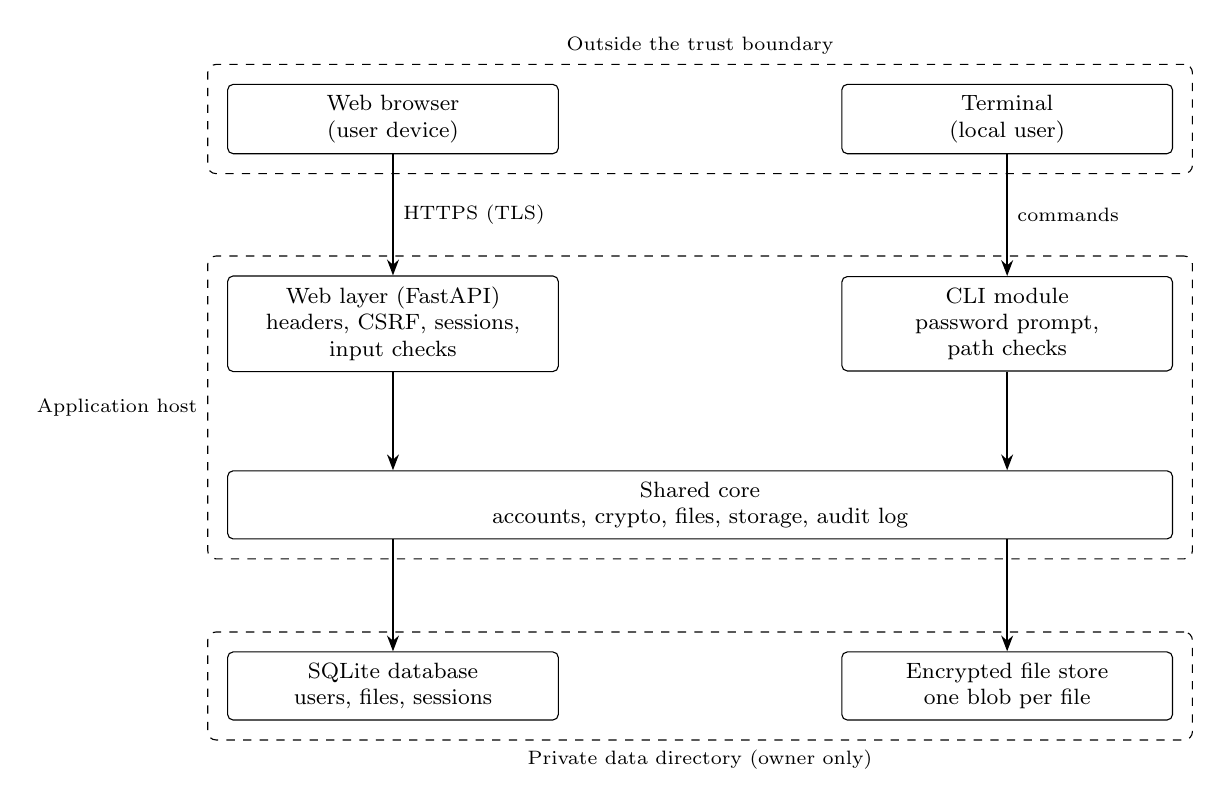
\begin{tikzpicture}
        \node[box, minimum width=4.2cm] (browser) at (0,0) {Web browser\\(user device)};
        \node[box, minimum width=4.2cm] (term) at (7.8,0) {Terminal\\(local user)};
        \node[box, minimum width=4.2cm] (web) at (0,-2.6) {Web layer (FastAPI)\\headers, CSRF, sessions,\\input checks};
        \node[box, minimum width=4.2cm] (clim) at (7.8,-2.6) {CLI module\\password prompt,\\path checks};
        \node[box, minimum width=12cm] (core) at (3.9,-4.9) {Shared core\\accounts, crypto, files, storage, audit log};
        \node[box, minimum width=4.2cm] (db) at (0,-7.2) {SQLite database\\users, files, sessions};
        \node[box, minimum width=4.2cm] (blobs) at (7.8,-7.2) {Encrypted file store\\one blob per file};
        \draw[arr] (browser) -- node[right, note] {HTTPS (TLS)} (web);
        \draw[arr] (term) -- node[right, note] {commands} (clim);
        \draw[arr] (web) -- (web |- core.north);
        \draw[arr] (clim) -- (clim |- core.north);
        \draw[arr] (db |- core.south) -- (db);
        \draw[arr] (blobs |- core.south) -- (blobs);
        \node[region, fit=(browser)(term), label={[note]above:Outside the trust boundary}] {};
        \node[region, fit=(web)(clim)(core), label={[note]left:Application host}] {};
        \node[region, fit=(db)(blobs), label={[note]below:Private data directory (owner only)}] {};
    \end{tikzpicture}
    \caption{System architecture and trust boundaries.}
    \label{fig:architecture}
\end{figure}

\section{Accounts and encryption keys}

A username has 1 to 64 characters: letters, digits, dot, underscore and hyphen. A password has 8 to 128 characters. The upper limit stops very long passwords from slowing down the server, because Argon2id needs much time and memory. The database stores a salted Argon2id hash of the password \cite{rfc9106, owaspPasswords}. It never stores the password.

Each user has a random 256-bit master key that encrypts the files of this user. The application does not store the master key in plain form. It encrypts the master key with a key-encryption key (KEK). The KEK comes from the password with a second Argon2id run and a separate random salt. Figure~\ref{fig:keys} shows this. A person who steals the database cannot decrypt the files without the password. The price is that there is no password recovery.

\begin{figure}[htb]
    \centering
    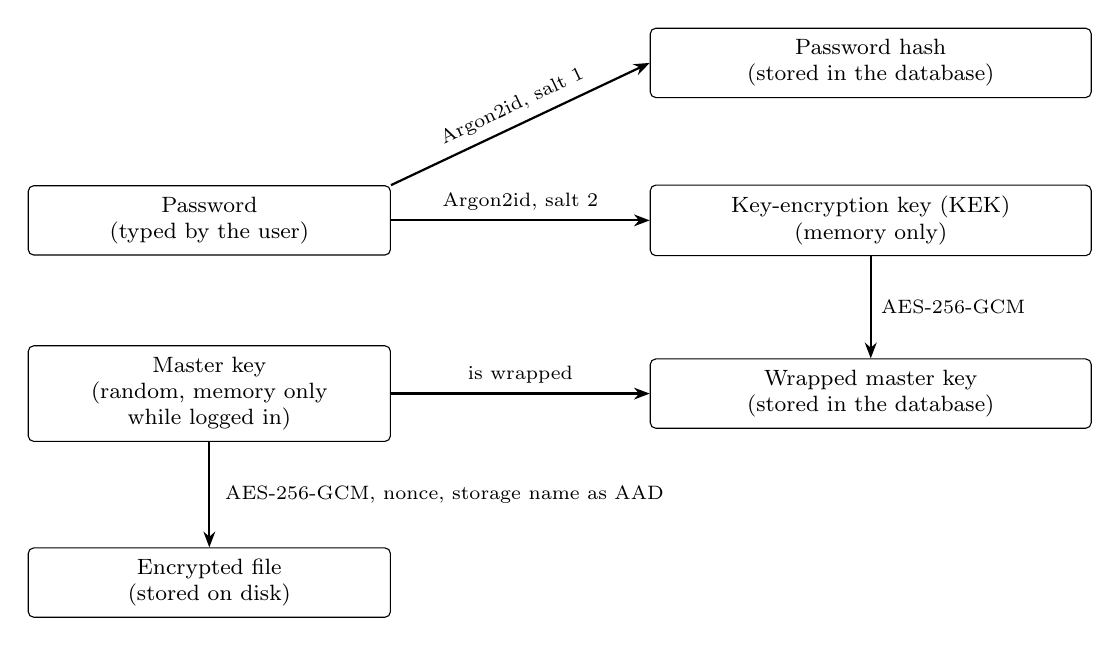
\begin{tikzpicture}
        \node[box, minimum width=4.6cm] (pw) at (0,0) {Password\\(typed by the user)};
        \node[box, minimum width=5.6cm] (hash) at (8.4,2.0) {Password hash\\(stored in the database)};
        \node[box, minimum width=5.6cm] (kek) at (8.4,0) {Key-encryption key (KEK)\\(memory only)};
        \node[box, minimum width=5.6cm] (wrapped) at (8.4,-2.2) {Wrapped master key\\(stored in the database)};
        \node[box, minimum width=4.6cm] (mk) at (0,-2.2) {Master key\\(random, memory only\\while logged in)};
        \node[box, minimum width=4.6cm] (blob) at (0,-4.6) {Encrypted file\\(stored on disk)};
        \draw[arr] (pw.north east) -- node[above, note, sloped, pos=0.5] {Argon2id, salt 1} (hash.west);
        \draw[arr] (pw) -- node[above, note] {Argon2id, salt 2} (kek);
        \draw[arr] (kek) -- node[right, note] {AES-256-GCM} (wrapped);
        \draw[arr] (mk) -- node[above, note] {is wrapped} (wrapped);
        \draw[arr] (mk) -- node[right, note, xshift=2pt] {AES-256-GCM, nonce, storage name as AAD} (blob);
    \end{tikzpicture}
    \caption{Key hierarchy. At login the KEK unlocks the master key again.}
    \label{fig:keys}
\end{figure}

Files use AES-256-GCM with a fresh random 12-byte nonce \cite{nistgcm}. The encrypted file holds the ciphertext followed by the 16-byte tag. The nonce is in the database. The random storage name of the file is part of the authenticated data, so an attacker cannot swap the content of two files. A changed file or a wrong key makes the decryption fail.

At login the application checks the password format, finds the user with a bound query, and verifies the password hash. For an unknown user it verifies against a dummy hash, so the response time does not show which usernames exist. Every failure returns the same message: ``Invalid username or password.'' Login and registration are limited to 10 requests in 5 minutes for each client address.

\section{Sessions and CSRF protection}

The web application keeps sessions on the server. The browser only holds a random 256-bit token in a cookie with the attributes Secure, HttpOnly and \texttt{SameSite=Strict} \cite{owaspSessions}. A new session is created at every login, and the old session of the browser is destroyed. This prevents session fixation. The idle timeout is 15 minutes, and the absolute lifetime is 12 hours. The unlocked master key stays in a cache in process memory. It is not in the database or in the cookie. After a server restart all users must log in again.

Every form that changes data has a hidden CSRF token \cite{owaspCsrf}. The login and registration forms use a single-use token that is linked to a short-lived \texttt{preauth} cookie. All other forms (upload, delete, logout) use a random token that belongs to the session. The server compares tokens in constant time. A request without a valid token gets the status 403. Requests that only read data do not change any state.

\section{XSS protection}

Jinja2 escapes all values in the HTML templates, for example file names. The templates do not use the \texttt{safe} filter and contain no JavaScript. Because of this, the Content Security Policy can forbid all scripts: \texttt{default-src 'self';} \texttt{script-src 'none';} \texttt{object-src 'none';} \texttt{base-uri 'none';} \texttt{frame-ancestors 'none';} \texttt{form-action 'self'}. A middleware function adds this header to every response. It also adds \texttt{X-Content-Type-Options: nosniff}, \texttt{X-Frame-Options: DENY}, \texttt{Referrer-Policy: no-referrer}, \texttt{Cache-Control: no-store} and HSTS \cite{rfc6797}. The application never shows file content in a page. Downloads have the type \texttt{application/octet-stream} and the header \texttt{Content-Disposition: attachment}.

\section{Input validation and uploads}

The server validates all input. The client checks help the user but give no protection. Table~\ref{tab:validation} lists the main rules.

\begin{longtable}[hp]{|p{3.0cm}|p{7.5cm}|p{2.6cm}|}
	\caption{Input validation rules.}
	\label{tab:validation}\\ \hline
	\textbf{Input} & \textbf{Rule} & \textbf{Where} \\
	\hline
	\endfirsthead
	\multicolumn{3}{l}{\tablename\ \thetable\ -- \textit{Continues...}} \\
	\hline
	\textbf{Input} & \textbf{Rule} & \textbf{Where} \\
	\hline
	\endhead
	\hline \multicolumn{3}{l}{\textit{Continues...}} \\
	\endfoot
	\hline
	\endlastfoot
	Username, password & Format and length as in Section 2.2. & Web, CLI, core \\ \hline
	Upload file name & Keep the part after the last \texttt{/} or backslash. Replace each character outside letters, digits, \texttt{.}, \texttt{\_}, space and \texttt{-} with \texttt{\_}. Cut to 255 characters. Reject empty names, \texttt{.} and \texttt{..}. & Web \\ \hline
	Upload type & Extension must be txt, md, csv, json, pdf, png, jpg, jpeg, zip or bin. & Web \\ \hline
	File size & At most 50 MiB. The code counts the bytes while it reads. & Web, CLI, core \\ \hline
	Stored name (CLI) & 1 to 255 characters from the safe set above. No path separators. & CLI, core \\ \hline
	File ID in a route & Must be an integer, or the status is 400. & Web \\ \hline
	Request size & At most 64 KiB, and for uploads 50 MiB plus 64 KiB. The server checks \texttt{Content-Length} and the real number of bytes. & Web \\ \hline
	Local path (CLI) & No \texttt{..} part, no control characters, no symbolic links. & CLI, core \\ \hline
\end{longtable}

The extension list is a simple policy. It is not a malware scan. This is acceptable here, because the application never runs, unpacks or shows an uploaded file \cite{owaspUpload}. The framework would write large uploads to a temporary file in plain form. The application sets the parser limit so that uploads stay in memory instead.

\section{Storage, download and access control}

An upload is encrypted in chunks of 1 MiB with one reusable buffer. The code creates the blob file with a new random name, \texttt{O\_EXCL}, \texttt{O\_NOFOLLOW} and the mode 0600. The database row is written after the blob is complete. If anything fails, the function rolls back and removes the blob. A download decrypts the whole file in memory first, so no byte leaves the server before the tag check has passed. Then it sends the data in chunks and wipes the buffer.

Every file operation uses the user ID from the server-side session, and the user cannot change it. The list, download and delete functions all filter the database rows by this ID. Figure~\ref{fig:access} shows the flow for a download. A file of another user and a file that does not exist give the same answer (404), so an attacker cannot learn which IDs exist. The core library repeats the owner check, so a new route that forgets it in the web layer is still safe. The command-line tool finds a file by name only inside the list of the logged-in user.

\begin{figure}[htb]
    \centering
    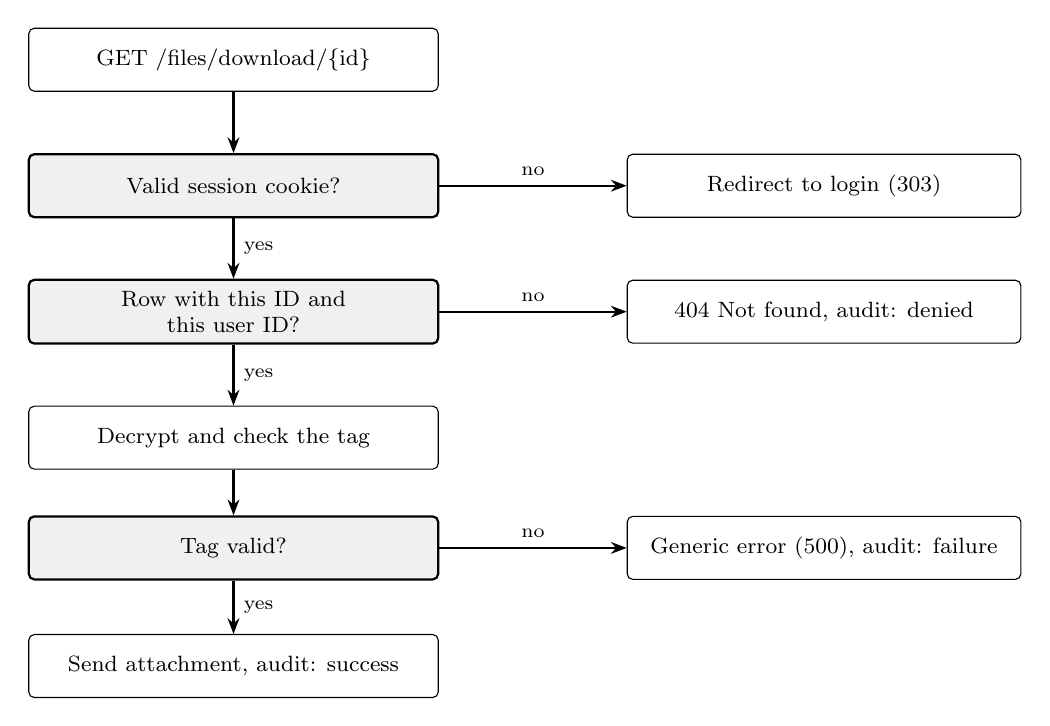
\begin{tikzpicture}
        \tikzset{decision/.style={box, thick, fill=gray!12, minimum width=5.2cm}}
        \node[box, minimum width=5.2cm] (start) at (0,0) {GET /files/download/\{id\}};
        \node[decision] (d1) at (0,-1.6) {Valid session cookie?};
        \node[decision] (d2) at (0,-3.2) {Row with this ID and\\this user ID?};
        \node[box, minimum width=5.2cm] (dec) at (0,-4.8) {Decrypt and check the tag};
        \node[decision] (d3) at (0,-6.2) {Tag valid?};
        \node[box, minimum width=5.2cm] (ok) at (0,-7.7) {Send attachment, audit: success};
        \node[box, minimum width=5cm] (r1) at (7.5,-1.6) {Redirect to login (303)};
        \node[box, minimum width=5cm] (r2) at (7.5,-3.2) {404 Not found, audit: denied};
        \node[box, minimum width=5cm] (r3) at (7.5,-6.2) {Generic error (500), audit: failure};
        \draw[arr] (start) -- (d1);
        \draw[arr] (d1) -- node[right, note] {yes} (d2);
        \draw[arr] (d2) -- node[right, note] {yes} (dec);
        \draw[arr] (dec) -- (d3);
        \draw[arr] (d3) -- node[right, note] {yes} (ok);
        \draw[arr] (d1) -- node[above, note] {no} (r1);
        \draw[arr] (d2) -- node[above, note] {no} (r2);
        \draw[arr] (d3) -- node[above, note] {no} (r3);
    \end{tikzpicture}
    \caption{Checks in a file download.}
    \label{fig:access}
\end{figure}

\section{SQL injection and file system safety}

The application uses the SQLAlchemy ORM for all queries, so user values go to the database as bound parameters, separate from the SQL text. The only direct SQL statement switches on the SQLite foreign key check and has no variable parts. The code never builds SQL text from input.

The module \texttt{core/storage.py} protects the file system. Blob names are random and are checked against a fixed pattern. The code opens a path one directory at a time with \texttt{O\_NOFOLLOW} and \texttt{O\_DIRECTORY}, so a symbolic link cannot replace a directory between the check and the use. It rejects \texttt{..} parts and control characters, checks with \texttt{fstat} that each opened file is a regular file, and rejects hard-linked files for overwrite and delete. Output files get the mode 0600 and never replace an existing file unless the user adds \texttt{-{}-force}. The data directory has the mode 0700. The source code has no shell call, so there is no command injection. I searched it for \texttt{subprocess}, \texttt{os.system}, \texttt{eval} and \texttt{exec} and found no use.

Secure deletion overwrites the whole file with zero bytes, flushes it, calls \texttt{fsync}, checks that the name still points to the same file, and then removes it. For a stored file it also removes the database row. The command-line tool asks for the password and a confirmation first. This is best effort. An SSD, a copy-on-write file system, a snapshot or a backup can keep old data.

\section{Memory management}

Pure Python code cannot cause a buffer overflow. The equivalent measures here are strict length limits on all input and bounded buffers. The second aim is to remove secrets from memory after use. The code keeps keys and file data in \texttt{bytearray} objects, which can be overwritten in place. The function \texttt{secure\_wipe} fills them with zeros in \texttt{finally} blocks, so it also runs after errors. The code wipes the KEK after use, the master key after registration and after each CLI command, each request copy of the master key, the key cache at logout, expiry and shutdown, the upload buffer and the plain data of a download. There are limits. A Python string such as the password cannot be overwritten, the crypto library returns \texttt{bytes} that the code cannot wipe, and the system can write memory to swap or to a crash dump.

\section{Errors, logging, TLS and secrets}

The user sees only fixed messages, such as ``Invalid request.'', ``Not found.'' and ``The request could not be completed.''. Three handlers (form errors, HTTP errors and a catch-all middleware) produce them, so no stack trace, path or database message reaches the user. The command-line tool prints \texttt{Error: The request could not be completed.} for unexpected errors and exits with the code 1.

The function \texttt{audit} writes one JSON object for each security event \cite{owaspLogging}. The fields are \texttt{timestamp} (UTC), \texttt{event} (from a fixed list such as \texttt{authentication}, \texttt{csrf}, \texttt{file\_encrypt}, \texttt{file\_decrypt}, \texttt{file\_delete}), \texttt{outcome} (\texttt{success}, \texttt{failure} or \texttt{denied}), \texttt{user\_id} and \texttt{source\_address}. The function accepts no free text and raises an error for an unknown event or outcome. The log never contains passwords, tokens, keys, file names, file content or exception text. A typical line is:

\begin{lstlisting}[frame=single, basicstyle=\scriptsize, breaklines=true]
{"timestamp": "2026-11-16T17:56:28.558538+00:00", "event": "file_decrypt", "outcome": "denied", "user_id": 2, "source_address": "127.0.0.1"}
\end{lstlisting}

The web server must run over HTTPS. The script \texttt{certs/generate\_cert.sh} makes a local certificate with \texttt{mkcert} or \texttt{openssl}, and Uvicorn loads it. The recommended command also uses \texttt{-{}-no-proxy-headers} and \texttt{-{}-no-access-log}, so clients cannot fake their address and access logs cannot leak query strings. The application needs very few secrets. It has no database password, API key or mail account, and each user key is stored only in wrapped form. The certificate, the private key, the \texttt{data/} directory, database files and \texttt{.env} are in \texttt{.gitignore}.


\chapter{Security Analysis}\label{chapter:results}
\section{Test method and results}

I used three methods. First, an automatic test suite checks the core library, the web application, the command-line tool and the TLS connection. The tests use their own temporary database, storage directory and certificate. Second, I attacked a running HTTPS server with a script, with two users, Alice and Bob. Third, I reviewed the source code for missing checks, shell calls, raw SQL and places where a secret could enter a log.

The suite has 53 tests in five files. All 53 passed, found no broken requirements. The tests cover CSRF, access control, SQL injection, XSS, upload types and sizes, path and link attacks, encryption and tampering, secure deletion, sessions and login failures, memory cleanup, log content, generic errors and a real HTTPS connection. The commands to repeat the run are:

\begin{lstlisting}[frame=single, basicstyle=\small, breaklines=true]
python3 -m venv .venv && source .venv/bin/activate
python -m pip install -r requirements-dev.txt
python -m pytest -v --junitxml=docs/checkpoint3-results.xml
\end{lstlisting}

\section{Attack demonstrations}

\textbf{CSRF.} The test signs in as Alice and uploads a file. It opens a second session and sends nine requests to the upload, delete and logout routes. Each route gets a request without a token, one with the text \texttt{forged-token} and one with the token of the second session. All nine return 403. The file stays in place and can be downloaded. After that, the valid token of Alice deletes the file. On the running server, an upload without a token and a delete with a forged token also returned 403.

\textbf{Access to the file of another user.} Alice uploads \texttt{notes.txt}. Bob does not see it in his list. Bob requests the download and delete routes with the ID of the file of Alice. For the delete request he uses his own valid CSRF token, so that only the owner check can stop him. Both return 404. In the command-line tool, Bob tries to decrypt and delete \texttt{notes.txt} by name. Both commands fail with exit code 1 and create no output. The blob stays on disk, and Alice can still use her file.

\section{Attack vectors and results}

Table~\ref{tab:attacks} lists the attack vectors that I tried, the observed result and the control that stopped each attack.

\begin{longtable}[hp]{|p{2.7cm}|p{7.5cm}|p{3.0cm}|}
	\caption{Attack vectors, results and mitigations.}
	\label{tab:attacks}\\ \hline
	\textbf{Attack} & \textbf{Attempt and observed result} & \textbf{Mitigation} \\
	\hline
	\endfirsthead
	\multicolumn{3}{l}{\tablename\ \thetable\ -- \textit{Continues...}} \\
	\hline
	\textbf{Attack} & \textbf{Attempt and observed result} & \textbf{Mitigation} \\
	\hline
	\endhead
	\hline \multicolumn{3}{l}{\textit{Continues...}} \\
	\endfoot
	\hline
	\endlastfoot
	CSRF & Missing, forged and other-session tokens returned 403 on upload, delete and logout. Missing, reused and expired login tokens were rejected. & Session and pre-login tokens, SameSite cookie. \\ \hline
	Cross-user access & Bob could not list, download, decrypt or delete the file of Alice (web 404, CLI exit code 1). & Owner filter in every operation. \\ \hline
	SQL injection & The payloads \texttt{' OR 1=1 -{}-}, \texttt{' UNION SELECT 1 -{}-} and \texttt{'; DROP TABLE files; -{}-} reached the queries only as bound parameters, and the SQL text had only \texttt{?} placeholders. No record was returned and no table was removed. A route ID \texttt{1 OR 1=1} returned 400. A login with \texttt{alice' OR 1=1 -{}-} returned 401. & ORM parameter binding, integer route IDs. \\ \hline
	XSS & The file name \texttt{<img src=x onerror=alert(1)>.txt} became \texttt{\_img src\_x onerror\_alert\_1\_\_.txt}. A script tag in stored metadata was shown as escaped text. A text file with a script tag was sent as an attachment. & Name cleaning, auto-escaping, CSP, download headers. \\ \hline
	Unsafe uploads & HTML, SVG, PHP, Python, executable and extensionless files returned 400 and created no record. A file of exactly 50 MiB was accepted. One more byte was rejected, and the partial blob was removed. & Extension list, size limits. \\ \hline
	Traversal and command injection & The names \texttt{test;touch pwn}, \texttt{../file}, \texttt{a/b} and \texttt{a\textbackslash b} were rejected. A \texttt{..} part and symbolic links in the parent path were refused for read, write and wipe. \texttt{/static/../core/db.py} returned 404. & Strict names, no shell, no-follow opens. \\ \hline
	Link attacks & A symbolic link in place of a blob could not be read or deleted. Files with hard links could not be overwritten or wiped. & Regular-file and link-count checks. \\ \hline
	Encryption failures & Empty and binary files made a correct round trip. A wrong key, changed ciphertext or wrong additional data made the decryption fail. No plain text was in the blob. & AES-GCM tag check. \\ \hline
	Deletion & Just before removal, the file contained only zero bytes. The database row was removed. & Overwrite, fsync, identity check. \\ \hline
	Login and session abuse & Wrong and unknown credentials gave the same message. The eleventh attempt in five minutes returned 429. Login created a new session. Logout and both expiry types removed the key from the cache. & Argon2id, rate limit, session lifecycle. \\ \hline
	Errors, secrets in logs, memory & Simulated storage and database errors gave a generic message. The captured log had no sample password, file content, token or key. Buffers were zero after success and after errors. & Fixed log format, error handlers, \texttt{finally} cleanup. \\ \hline
	TLS and headers & A real HTTPS request succeeded with certificate verification. The response had secure cookies, the CSP and HSTS. & Uvicorn TLS, middleware. \\ \hline
\end{longtable}

\chapter{Conclusion}\label{chapter:discussion}
The file manager has a web interface and a command-line tool on one core library. It encrypts all files with AES-256-GCM, protects keys with Argon2id, and uses HTTPS, CSRF tokens, a strict CSP, bound SQL parameters and owner checks on every file operation. I tested these controls with 53 automatic tests and with attacks on a running server. All tests passed, and all attacks failed.

The application has limits. The server sees the plain file during use, because the encryption runs on the server. Memory wiping and secure deletion are best-effort measures: Python and the library can keep copies, and SSDs, snapshots and backups can keep old data. The key cache, the pre-login tokens and the rate limit are in the memory of one process, so the server must run with one worker. The rate limit works per client address and has no lockout for one account. There is no multi-factor authentication and no password recovery. The application checks only the extension of an upload, and it does not scan files for malware. Behind a reverse proxy, the trusted proxy addresses and the rate limits must be configured, and request bodies, cookies and query strings must not be logged.

I learned three main lessons. First, a shared core library keeps the ownership checks the same in the web layer and in the CLI. Second, encrypted data must be checked before it is used, and error paths need as much care as normal paths: many bugs were in cleanup code after an error. Third, a check before opening a file is not enough, and the code must check the file that it really opened. The main challenges were to keep plain data in memory small for files up to 50 MiB, to update the libraries without changing the web behavior, and to test deletion and cleanup.


\zlabel{lastpagetocount}        % DO NOT REMOVE! Used for counting number of pages of main text


\pagebreak % Content that follows starts on the new page
\phantomsection % Creates linkable section without placing visible content
\addcontentsline{toc}{chapter}{\referencesTitle} % adds a new chapter entry labeled "Kasutatud kirjandus" to TOC
\printbibliography[title=\referencesTitle] % The command pulls from the .bib file and and formats the output

\end{document}
